% ====================================================================
%+
% SECTION:
%    SolarSystem_Discovery.tex
%
% CHAPTER:
%    solarsystem.tex
%
% ELEVATOR PITCH:
%    Discovery of solar system objects, especially NEOs but others too.
%    Figure of merit is completeness.
%
%-
% ====================================================================

\section{Discovery: Linking Solar System Objects}
\def\secname{\chpname:discovery}\label{sec:\secname}

\credit{rhiannonlynne},
\credit{davidtrilling},
\credit{ivezic}

Discovering, rather than simply detecting, small objects throughout
the Solar System requires unambiguously linking a series of detections
together into an orbit. The orbit provides the information necessary
to scientifically characterize the object itself and to understand the
population as a whole. Without orbits, the detections of Solar System
Objects (SSOs) by LSST will be of limited use; objects discovered with
other facilities could be followed up by LSST, but almost the entire
science benefit to planetary astronomy would be lost. Linking and
orbit determination for Solar System objects is similar to source
association for non-moving objects; it provides the means to identify
multiple detections as coming from a single object.

Therefore, the first concern regarding the Solar System is related
to the question ``Can we accurately link individual detections of moving objects into
orbits?''.  This requirement poses varying levels of difficulty as we
move from Near Earth Objects (NEOs) through the Main Belt Asteroids
(MBAs) and to Trans-Neptunian Objects (TNOs) and Scattered Disk Objects
(SDOs), as well as for comets and for other unusual but very
interesting populations such as Earth minimoons. Due to their small
heliocentric and geocentric distances, NEOs appear to move with
relatively high velocities and are distributed over a large fraction
of the sky, including regions far from the ecliptic plane. MBAs are densely distributed,
primarily within about 30 degrees of the ecliptic. TNOs and SDOs move
slowly, however short time intervals between repeat visits in each night may make these difficult
to link. Comets and Earth mini-moons may require more complicated
orbit fitting to allow for non-gravitational or geocentric
orbits. The requirements of accurately linking individual detections
into orbits also implies that we do not create false objects by
incorrectly linking detections and/or noise.

Much of the answer to this question comes down to the performance of
various pieces of LSST Data Management software. In particular,
important questions are the
rate of false positive detections resulting from difference imaging, possible
limitations of the Moving Object Processing System (MOPS) to extend to high
apparent velocities, and the capability to unambiguously determine if
a linkage is `real' or not via orbit determination (done as part of
MOPS). Thus this question includes concerns beyond the limits of the OpSim simulated
surveys, although it still bears on the observing strategy requirements for
discovering Solar System Objects. An in-depth study of the performance
of difference imaging and MOPS is currently ongoing. However, we can
make a range of assumptions on how MOPS will perform and evaluate how
many and which objects can be linked under observational cadence, given those assumptions.


% --------------------------------------------------------------------

\subsection{Target measurements and discoveries}
\label{sec:\secname:targets}

The criteria for `discovery' with MOPS depends on the number
of observations of an object acquired per night within some time
window (creating `tracklets'), repeated over a number of nights within window of some
days (creating `tracks'), which are then linked into an orbit with a threshold on
astrometric residuals. The current assumptions are that we can link
detections into orbits with 2 detections per night within 90 minutes,
repeated for 3 nights within a window of 15 days. The additional assumptions are
that with these 6 observations, we will be able to create low-accuracy orbits that will suffice to link
additional observations obtained at later (or earlier, in the LSST
archive) times, and that that the orbit fitting will enable rejection
of mislinkages.

We can also use other requirements for discovery. Requiring 4
detections in each night is a fairly common discovery criteria for
NEO surveys, as it reduces the number of mislinked tracklets to almost
zero. We could also require 4 nights of pairs within a window of 20 days, in order to improve the
initial orbit fitting and mislinkage rejection. We can also assume
MOPS will perform better than the current assumptions, and evaluate
discovery criteria of 3 pairs within a 30 day window.

With these discovery criteria, we can then evaluate the completeness
of an LSST simulated survey, for a given population. We can look at
this as a function of H magnitude and as a function of orbital
parameters.

For PHAs and NEOs there are special considerations in terms of
completion that arise from planetary defense concerns. For most other
populations, the general desire is simply to have a high level of
completeness, with no gaps in completeness that depend strongly on
orbital parameters. In particular, the desire is to be able to
calibrate any selection effects in discovery so that the survey completeness can
be used to debias the underlying population models.

Discovery opportunity, and thus the completeness of the underlying
population, is very sensitive to the time interval between
observations. Waiting longer between observations within a night means that objects
may move beyond a single LSST field of view. Longer times between
revisits means that observing in large contiguous blocks (rather than
narrow, disconnected strips) within a night becomes more important to make sure that
objects are followed between pointings, especially if the time
interval is much longer than 30 minutes. Because the objects must be
detected on several nights within the window, the inter-night revisit
rate for similar large contiguous blocks of sky is important.

An optimal discovery strategy for moving
objects could be ensuring a minimum (default: two) number of revisits
within a night within a short time window (default: 90 minutes),
preferably over a large block of sky, and
covering large contiguous amounts of sky several (default: 3) times within a
longer time window (default: 15 days).  Observations within a single
night do not need to be in the same filter, however we will be
constrained by the shallower limiting magnitude of the pair; {\it e.g.}
preferably $r$ band observations would be paired with $i$ rather than
$u$ observations. Finally, the fill factor of the camera is important;
in these simulations we have used the LSST focal plane, which has an
approximately 92\% fill factor.

% --------------------------------------------------------------------

\subsection{Metrics}
\label{sec:\secname:metrics}

The {\tt DiscoveryChancesMetric} can be used to identify sets of detections
of a particular object that meet the defined criteria for discovery: X
detections within T minutes in a night, Y nights within a W day
window; this describes the number of discovery opportunities for each object. The results from the Discovery Metric can be fed to the {\tt
  MoCompletenessMetric} summary metric, where if an object achieves a
user-defined requirement for the minimum number of discovery
opportunities (typically 1), then it is counted as `discovered'.
The total number of objects discovered at each H magnitude is compared
to the total number of objects in the population at that H magnitude,
in order to evaluate `completeness' as a function of H. Discovery
opportunities can be evaluated as a function of orbital parameters, to
look for areas of orbital space that may be missed in a particular
survey strategy; completeness, since it marginalizes over the entire
population at a particular H value, loses this
capability. Completeness can be evaluated as a differential value
(completeness @ H=X) or integrated over the size distribution
(completeness @ H $\leq$ X).

The completeness can be parametrized by the completeness ($C_b$) at
some bright absolute magnitude ($H_b$), combined with the magnitude at
which this falls to 50\% ($H_f$). A draft set of requirements for
these parameters has been written up in the Solar System Object
Specifications document, although these requirements are still quite
preliminary. The current goal parameters are described in Table~\ref{ssoreqs}.

\begin{table}[]
\centering
\caption{Solar System Object Differential Completeness Goals}
\label{ssoreqs}
\begin{tabular}{llll}
    & $C_b$ & $H_b$ & $H_f$ \\
NEA & 80\%  & 18.4  & 21.9  \\
MBA & 90\%  & 19.5  & 20.2  \\
TNO & 90\%  & 7.0   & 8.1
\end{tabular}
\end{table}

A further simplification of the completeness can be achieved by simply
measuring the completeness at a preset absolute magnitude. For
example, completeness for PHAs at H=22 is an important summary value.


% --------------------------------------------------------------------

\subsection{OpSim Analysis}
\label{sec:\secname:analysis}

The basic output from the {\tt DiscoveryChancesMetric} is the number
of discovery opportunities (e.g. sets of observations that match the
required discovery criteria) available. For objects which have at
least a given number of discovery opportunities (here, we simply use
one required opportunity), then this object can be considered
``found'' and marked towards the completeness of the population at a
given H magnitude with the {\tt MoCompletenessMetric} summary metric.
Examining the \opsimdbref{db:baseCadence} with these metrics, we find
that most objects have many discovery opportunities. This is shown in
Figure~\ref{standard_discovery}.

\begin{figure}
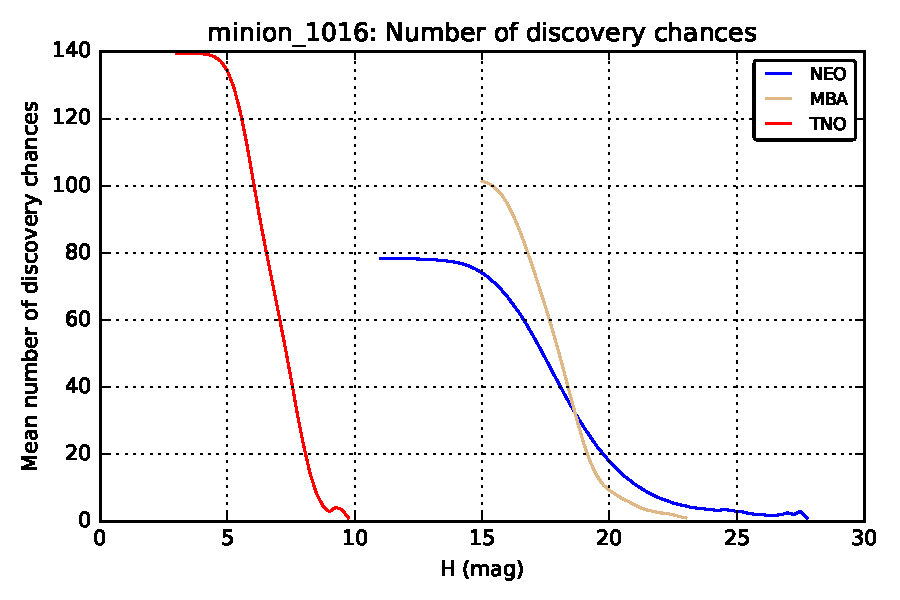
\includegraphics[width=3.3in]{figs/solarsystem/minion_1016_DiscoveryChances_tno_mba_neo_10_year_3_pairs_in_15_nights_MOOB_ComboMetricVsH}
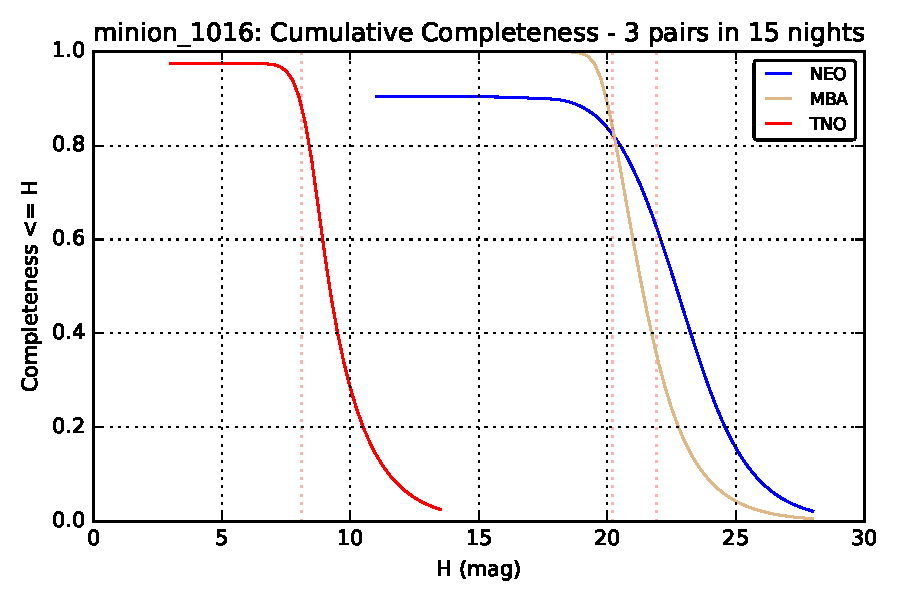
\includegraphics[width=3.3in]{figs/solarsystem/minion_1016_CumulativeCompleteness_tno_mba_neo_10_year_3_pairs_in_15_nights_MOOB_ComboMetricVsH}
\caption{Left: Number of discovery chances as a function of H
  (mean value for all objects at each $H$ value), assuming the minimum criteria for
  discovery - 2 visits per night within 90 minutes, repeated for 3
  nights within 15 days. Right: Resulting cumulative completeness for
  each population, assuming that only 1 discovery opportunity is
  required to `discover' each object.
\label{standard_discovery}}
\end{figure}

The runs \opsimdbref{db:baseCadence}, \opsimdbref{db:NoVisitPairs},
\opsimdbref{db:NEOswithVisitTriplets}, \opsimdbref{db:NEOwithVisitQuads}
are particularly interesting to evaluate in light of the different
sets of discovery criteria. Because Opsim does not currently require
only pairs (or singles, triplets or quads), but instead will sometimes
acquire more than the requested number of visits, changing the
discovery criteria from pairs within a night to triplets or quads,
does not automatically cause the completeness to pummet, although it
does decrease. Looking at the raw numbers of discovery chances offers some
enlightenment: the number of discovery opportunities does falls dramatically as we go from pairs to quads, however, there
are still some times when observations are obtained in triplets or
quads, so there are still some discovery chances. This behavior of the
scheduler (to frequently acquire more than the requested number of
visits) is likely to change in the future and make this effect more pronounced, but the completeness will
clearly be very sensitive to how observations are acquired. This effect is shown in
Figure~\ref{completeness_changes}.

\begin{figure}
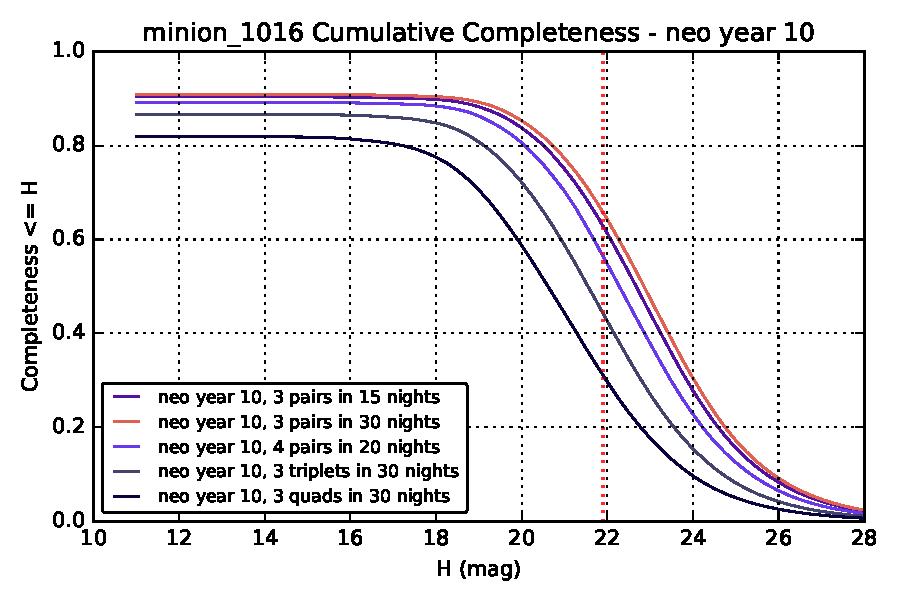
\includegraphics[width=3.3in]{figs/solarsystem/minion_1016_CumulativeCompleteness_pairs_20_4_quads_3_30_3_30_triplets_3_30_pairs_3_15_pairs_nights_in_neo_year_10_MOOB_ComboMetricVsH}
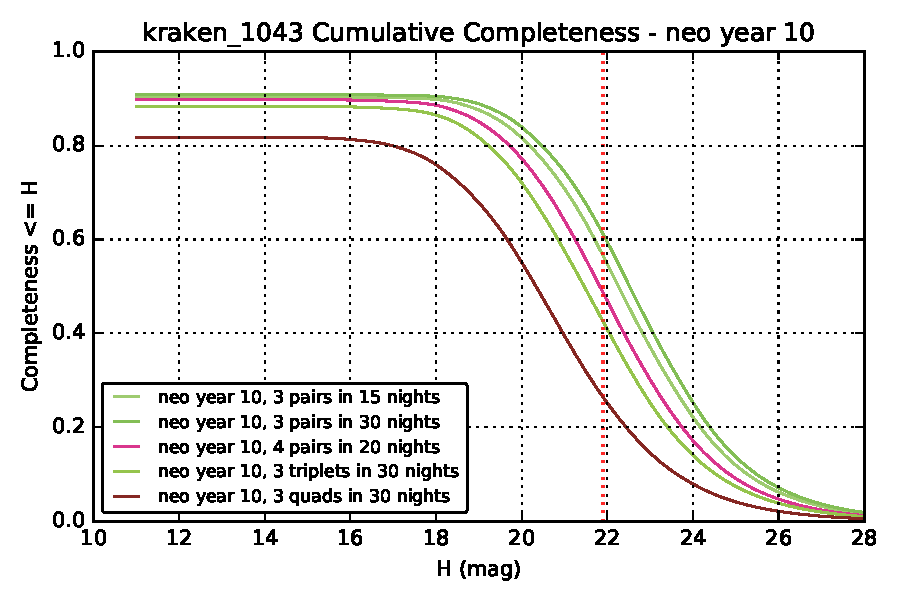
\includegraphics[width=3.3in]{figs/solarsystem/kraken_1043_CumulativeCompleteness_pairs_20_4_quads_3_30_3_30_triplets_3_30_pairs_3_15_pairs_nights_in_neo_year_10_MOOB_ComboMetricVsH} \\
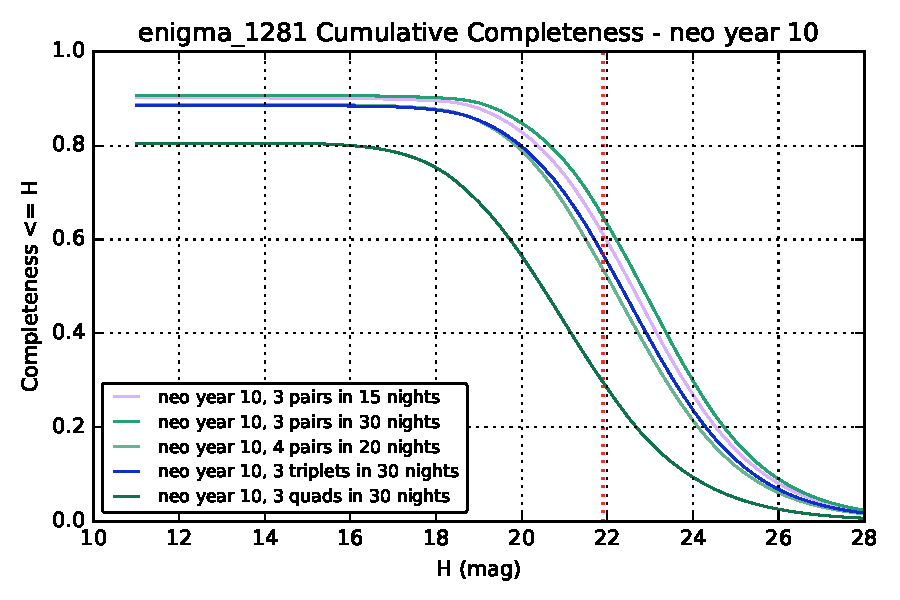
\includegraphics[width=3.3in]{figs/solarsystem/enigma_1281_CumulativeCompleteness_pairs_20_4_quads_3_30_3_30_triplets_3_30_pairs_3_15_pairs_nights_in_neo_year_10_MOOB_ComboMetricVsH}
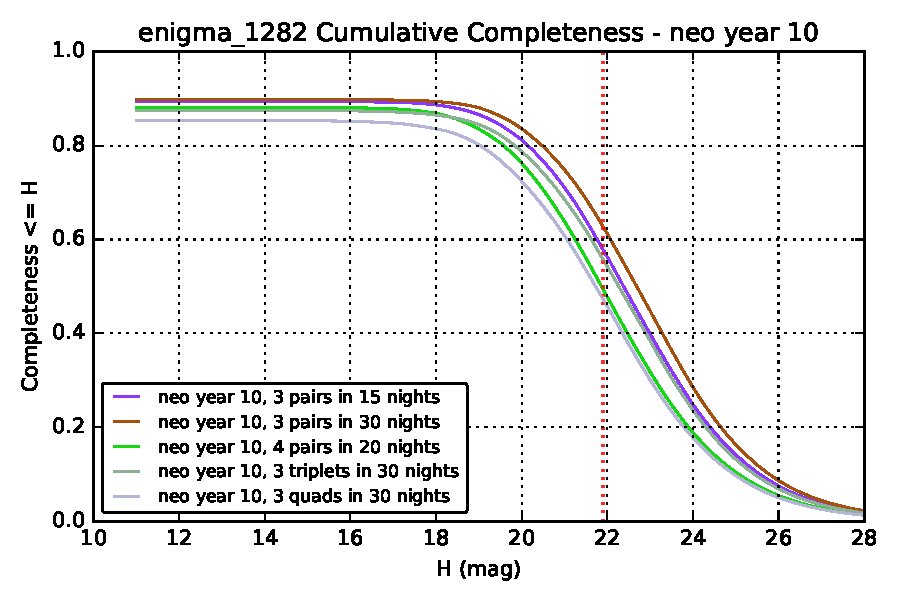
\includegraphics[width=3.3in]{figs/solarsystem/enigma_1282_CumulativeCompleteness_pairs_20_4_quads_3_30_3_30_triplets_3_30_pairs_3_15_pairs_nights_in_neo_year_10_MOOB_ComboMetricVsH}
\caption{Cumulative completeness for an NEO population, given
  different sets of discovery criteria, for the \opsimdbref{db:baseCadence}, \opsimdbref{db:NoVisitPairs},
\opsimdbref{db:NEOswithVisitTriplets},
\opsimdbref{db:NEOwithVisitQuads} simulated surveys. The results in the
lower right come from a simulated survey, \opsimdbref{db:NEOwithVisitQuads},
which attempted to obtain four visits to each field in each
night; the results on the upper left, come from the baseline simulated
survey, \opsimdbref{db:baseCadence}, which attempts to obtain pairs of
visits.
\label{completeness_changes}}
\end{figure}

Another aspect to consider is to look at how the completeness
increases over time. The completeness as a function of time is plotted
for particular $H$ values, depending on the
population, in Figure~\ref{completeness_time}.

\begin{figure}
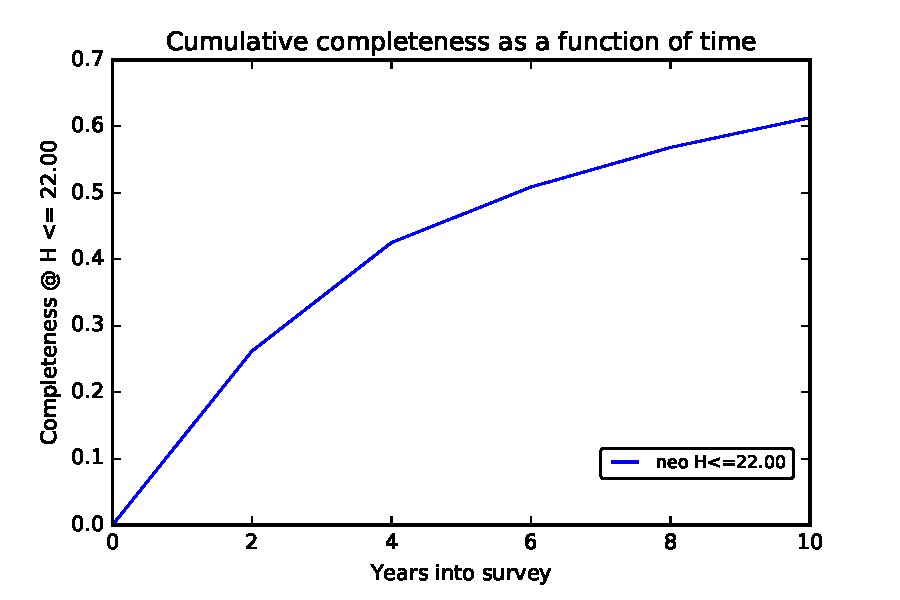
\includegraphics[width=2in]{figs/solarsystem/minion_1016_neo_CompletenessOverTime_22_time}
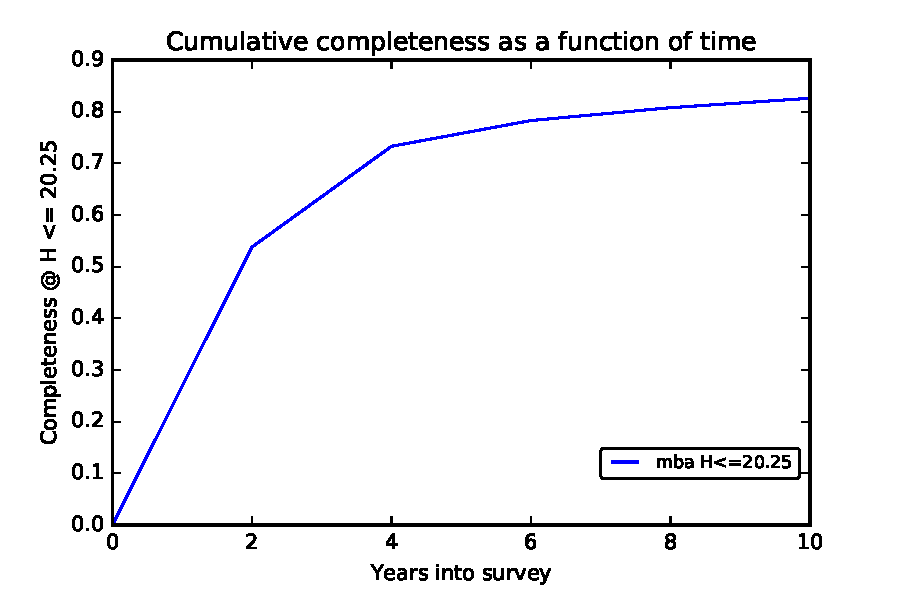
\includegraphics[width=2in]{figs/solarsystem/minion_1016_mba_CompletenessOverTime_20_time}
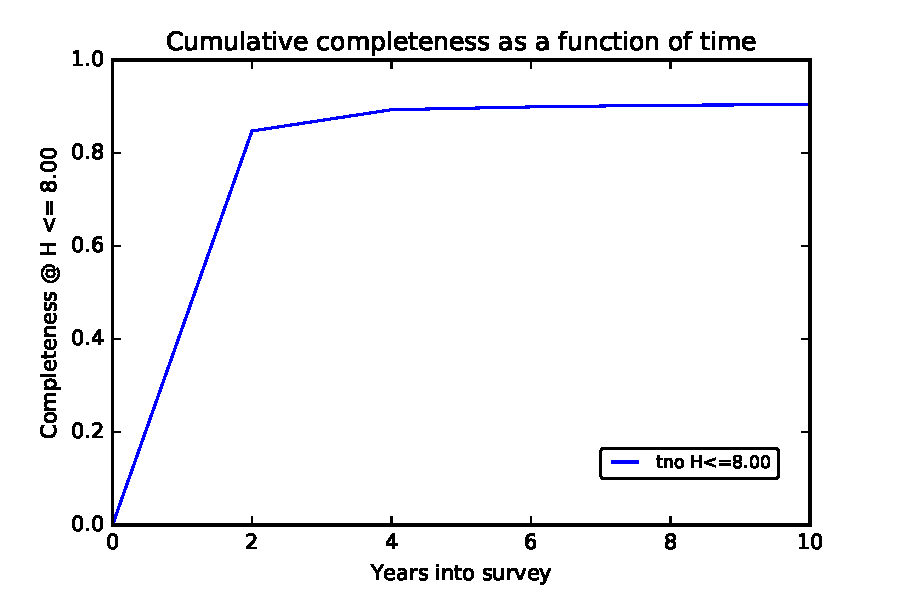
\includegraphics[width=2in]{figs/solarsystem/minion_1016_tno_CompletenessOverTime_8_time}
\caption{Completeness as a function of time, for NEO, MBA and TNO
  populations. The completeness increases rapidly for the first few
  years, then increases more slowly. The NEO completeness rises more
  slowly than other populations, as more NEOs become available to
  discover due to changing their orbital positioning relative to Earth
  (becoming closer and brighter, or moving away from sightlines behind
  the Sun). The TNO completeness rises most rapidly with time, as
  these objects move slowly; we find most of these objects within the
  first two years and then improve their characterization over the
  rest of the survey (measuring better orbits and obtaining
  lightcurves and colors).
\label{completeness_time}}
\end{figure}

\begin{table}[]
\centering
\caption{Solar System Object Differential Completeness in \opsimdbref{db:baseCadence}}
\label{ssoperf}
\begin{tabular}{llll}
    & $C_b$ & $H_b$ & $H_f$ \\
NEA & 87.5\%  & 18.5  & 21.5  \\
MBA & 89\%  & 19.5  & 20.2  \\
TNO & 96\%  & 7.0   & 8.3
\end{tabular}
\end{table}



% --------------------------------------------------------------------

\subsection{Discussion}
\label{sec:\secname:discussion}

A large portion of the risk in being able to discover moving objects
lies in the currently uncertain performance of the MOPS
software. Figure~\ref{completeness_changes} clearly shows that with
the baseline cadence, if we must have triplets or pairs, or even just
require 4 pairs of observations over 20 nights, that the completeness
falls. The performance will likely fall even further if the scheduler
stops obtaining more than the minimum requested number of observations.

With the expected MOPS discovery requirements,
\opsimdbref{db:baseCadence} performs adequately for most solar system
objects, although completeness falls off more rapidly for faint
objects than desired for NEOs. To investigate this effect, more
metrics will have to be developed to discover why these fainter NEOs
are not being discovered (are they simply missing appropriate
sequences of observations due to the cadence or is something more
subtle occuring?).

% --------------------------------------------------------------------
% PJM: the following content was moved from Chapter 2, before Lynne
% checked in a new analysis. I have commented out the old Chapter 2
% work for now.
%
% \subsection{OpSim Analysis of NEO/PHA completeness}
% \label{sec:\secname:analysis}
%
% %
% % \section{Analysis}
% % \def\secname{cadexp:NEOs}\label{sec:\secname}
%
% % \noindent{\it Analysis of NEO/PHA completeness:   ops2\_1094, enigma\_1258, enigma\_1259}
%
% Continuing the analysis of some alternatives to the Baseline Cadence
% started in \autoref{chp:cadexp},
% we now investigate a suite of observing strategies for their
% suitability in supporting Near-Earth Object (NEO) science. As in
% that chapter,
% % the previous section,
% these \OpSim databases are all available for further
% testing with science-based MAF metrics.
%
% The U.S. Congress has given a mandate to NASA to implement a
% Near-Earth Object (NEO) Survey program to detect, track, catalog,
% and characterize the physical characteristics of near-Earth objects
% equal to or greater than 140 meters in diameter\footnote{See
% \url{http://www.gpo.gov/fdsys/pkg/PLAW-109publ155/pdf/PLAW-109publ155.pdf}}.
% The goal is to achieve a completeness of 90\%. In recent practice,
% adopted here, the completeness is evaluated for a subset of NEOs
% called Potentially Hazardous Asteroids\footnote{Potentially Hazardous
% Asteroids (PHAs) are defined as asteroids with a minimum orbit
% intersection distance (MOID) of 0.05 AU or less.}  (PHA), with
% H$\le$22, where H is the absolute magnitude\footnote{Absolute
% magnitude is the magnitude that an asteroid would have at a distance
% of 1 AU from the Sun and from the Earth, viewed at zero phase angle.
% This is an impossible configuration, of course, but the definition is
% motivated by desire to separate asteroid physical characteristics from
% the observing configuration.} in the Johnson's V band. While LSST is
% very competitive in this context, it will also enable analysis of many
% other Solar System populations (e.g.\ main-belt asteroids, comets,
% trans-Neptunian objects). Nevertheless, we focus our analysis here on
% NEOs/PHAs completeness.
%
%
% {\bf Motivation and description:}\\
% The baseline cadence implements observing strategy with two visits to
% a field obtained per night, separated in time by a fraction of an
% hour. Motivation for a simulation that does require pairs of visits is
% to gauge its impact on the survey efficiency and other performance
% parameters. Motivation for simulations with more than two visits to a
% given field per night is to investigate the feasibility of a more
% robust approach to linking individual detections into a plausible
% object track. Although detailed simulations of the performance of
% image differencing software and orbital determination software
% indicate that two visits per night are likely to be sufficient,
% quantitative analysis of other strategies is clearly within the
% purview of the cadence optimization program.  Five simulations are
% analyzed in this section:
%
%
% % - - - - - - - - - - - - - - - - - - - - - - - - - - - - - - - - - -
%
% %%%%%%%%%%%%%%%%%%%%%%%%%%%%%%%%%%%%%%%%%%%
% \opsimdb[db:NEOsNoVisitPairs]{kraken\_1043}{NEO test: no request for pairs of visits.}
% %%%%%%%%%%%%%%%%%%%%%%%%%%%%%%%%%%%%%%%%%%%
%
% % - - - - - - - - - - - - - - - - - - - - - - - - - - - - - - - - - -
%
% %%%%%%%%%%%%%%%%%%%%%%%%%%%%%%%%%%%%%%%%%%%
% \opsimdb[db:NEOswithVisitPairs]{enigma\_1016}{NEO test: pairs of visits (i.e.\ the Baseline Cadence).}.
% %%%%%%%%%%%%%%%%%%%%%%%%%%%%%%%%%%%%%%%%%%%
%
% % - - - - - - - - - - - - - - - - - - - - - - - - - - - - - - - - - -
%
% %%%%%%%%%%%%%%%%%%%%%%%%%%%%%%%%%%%%%%%%%%%
% \opsimdb[db:NEOswithVisitTriplets]{enigma\_1281}{NEO test: triplets of visits.}
% %%%%%%%%%%%%%%%%%%%%%%%%%%%%%%%%%%%%%%%%%%%
%
% % - - - - - - - - - - - - - - - - - - - - - - - - - - - - - - - - - -
%
% %%%%%%%%%%%%%%%%%%%%%%%%%%%%%%%%%%%%%%%%%%%
% \opsimdb[db:NEOwithVisitQuads]{enigma\_1282}{NEO test: quads of visits.}
% %%%%%%%%%%%%%%%%%%%%%%%%%%%%%%%%%%%%%%%%%%%
%
% % - - - - - - - - - - - - - - - - - - - - - - - - - - - - - - - - - -
%
% {\bf Expectations:}  Analysis of all simulations is repeated three
% times, with different conditions for what constitutes an object's
% ``discovery'':  two, three or four detections per night are required,
% together with at least three such sequences in a 15-day window.  When
% only two detections per night are required, a modest decrease in PHA
% completeness is expected for simulations that request more than two
% visits per night because some visits ``don't live up to their full
% potential''. On the other hand, when more than two detections per
% night are required, a naive expectation is that PHA completeness for
% runs with fewer requested visits will drop significantly. \\
%
%
% %%%%%%%%%%%%%%%%%%%%%%%%%%%
% \begin{figure}[t!]
% \vskip -1.1in
% \includegraphics[angle=0,width=0.56\hsize:,clip]{figs/enigma1189_diffNEOcompleteness.pdf}
% \hskip -0.5in
% \includegraphics[angle=0,width=0.56\hsize:,clip]{figs/enigma1189_cumNEOcompleteness.pdf}
% \vskip -1.2in
% \caption{The PHA completeness for \opsimdbref{db:baseCadence}, as a function of the object's absolute
% visual magnitude H on the horizontal axes (left: differential completeness at a given H;
% right: cumulative completeness for all objects brighter than a given H).
% The completeness for H$\le$22 NEOs (those with diameters larger than 140m)  for this
% simulation is 73\% (blue line in the right panel). The panels also show the effects of ignoring
% chip gaps (a 2\% effect for cumulative H$\le$22 completeness) and of decreasing the
% field-of-view size to a half (i.e.\ to 4.8 sq.\ deg; a 10\% effect).}
% \label{fig:enigmaNEO}
% \end{figure}
% %%%%%%%%%%%%%%%%%%%%%%%%%%%
%
% %%%%%%%%%%%%%%%%%%%%%%%%%%%
% \begin{figure}[th!]
% \vskip -1.2in
% \includegraphics[angle=0,width=0.49\hsize:,clip]{figs/diffNEOpairs.pdf}
% \includegraphics[angle=0,width=0.49\hsize:,clip]{figs/diffNEOquads.pdf}
% \vskip -1.3in
% \caption{%
% The comparison of differential PHA completeness for the five analyzed simulations
% when requiring two detections per night (left) and four detections per night (right).
% With two detections per night, all simulations perform similarly but when four
% detections per night are required, the simulation that has the largest number
% of such sequences (see \autoref{fig:NvisitStats}), performs the best although at an
% inferior level compared to the left panel (see also \autoref{fig:enigmaNEO}).}
% \label{fig:NEOquads}
% \end{figure}
% %%%%%%%%%%%%%%%%%%%%%%%%%%%
%
%
% {\bf Analysis Results:}
%
% For baseline reference, the PHA completeness for
% \opsimdbref{db:baseCadence} is shown in \autoref{fig:enigmaNEO}. The
% baseline cadence achieves a cumulative completeness of 73\% for
% H$\le$22 PHAs. This cumulative completeness for H$\le$22 is 17\%
% higher than differential completeness at H=22 of 56\% due to
% increasing completeness towards smaller H (larger objects). Both
% differential and cumulative completeness are relevant metrics: the
% former provides more insight in the behavior of a particular
% simulation, while the latter is a metric given to NASA by the U.S.
% Congress. Analysis of results illustrated in \autoref{fig:NEOquads}
% can be summarized as follows:
% \begin{itemize}
% \item When NEO discovery algorithm requires pairs of visits, all runs
% have very similar PHA completeness, with quads run only about 2\%
% lower than the baseline (a differential completeness of 56\% at H=22
% for \opsimdbref{db:baseCadence})
% \item When NEO discovery algorithm requires 4 detections per night,
% the simulation with quads achieves a differential completeness of
% about 27\% at H=22, or  about 30\% lower completeness than Baseline
% Cadence.
% \item When NEO discovery algorithm requires 4 detections per night,
% Baseline Cadence reaches a differential completeness of about 15\% at
% H=22 (some quads are unintentionally produced by chance, see
% \autoref{fig:NvisitStats}).
% \item When NEO discovery algorithm requires 3 detections per night,
% runs which requested triples and quads achieve a differential
% completeness of about 40\% at H=22 (corresponding to a cumulative
% completeness of about 57\% for H$\le$22).
% \end{itemize}
%
% Therefore, going from pairs of visits to triples (both for cadence and
% NEO detection) reduces completeness (both differential and cumulative)
% for PHAs with H$\le$22 by about 15-20\% (and by about 30\% for quads).
%
%


\navigationbar
